\begin{frame}
	\frametitle{$C_{1}$: Knowledge-based Approach for Video Indexing}
	\begin{itemize}
	  \small
	  \item $C_{1}$ : A \alert{Knowledge-Based} Framework for video Indexing,
	  \item Capitalize on Semantic \alert{Concepts/Contexts relationships}.
	\end{itemize}
	\begin{center}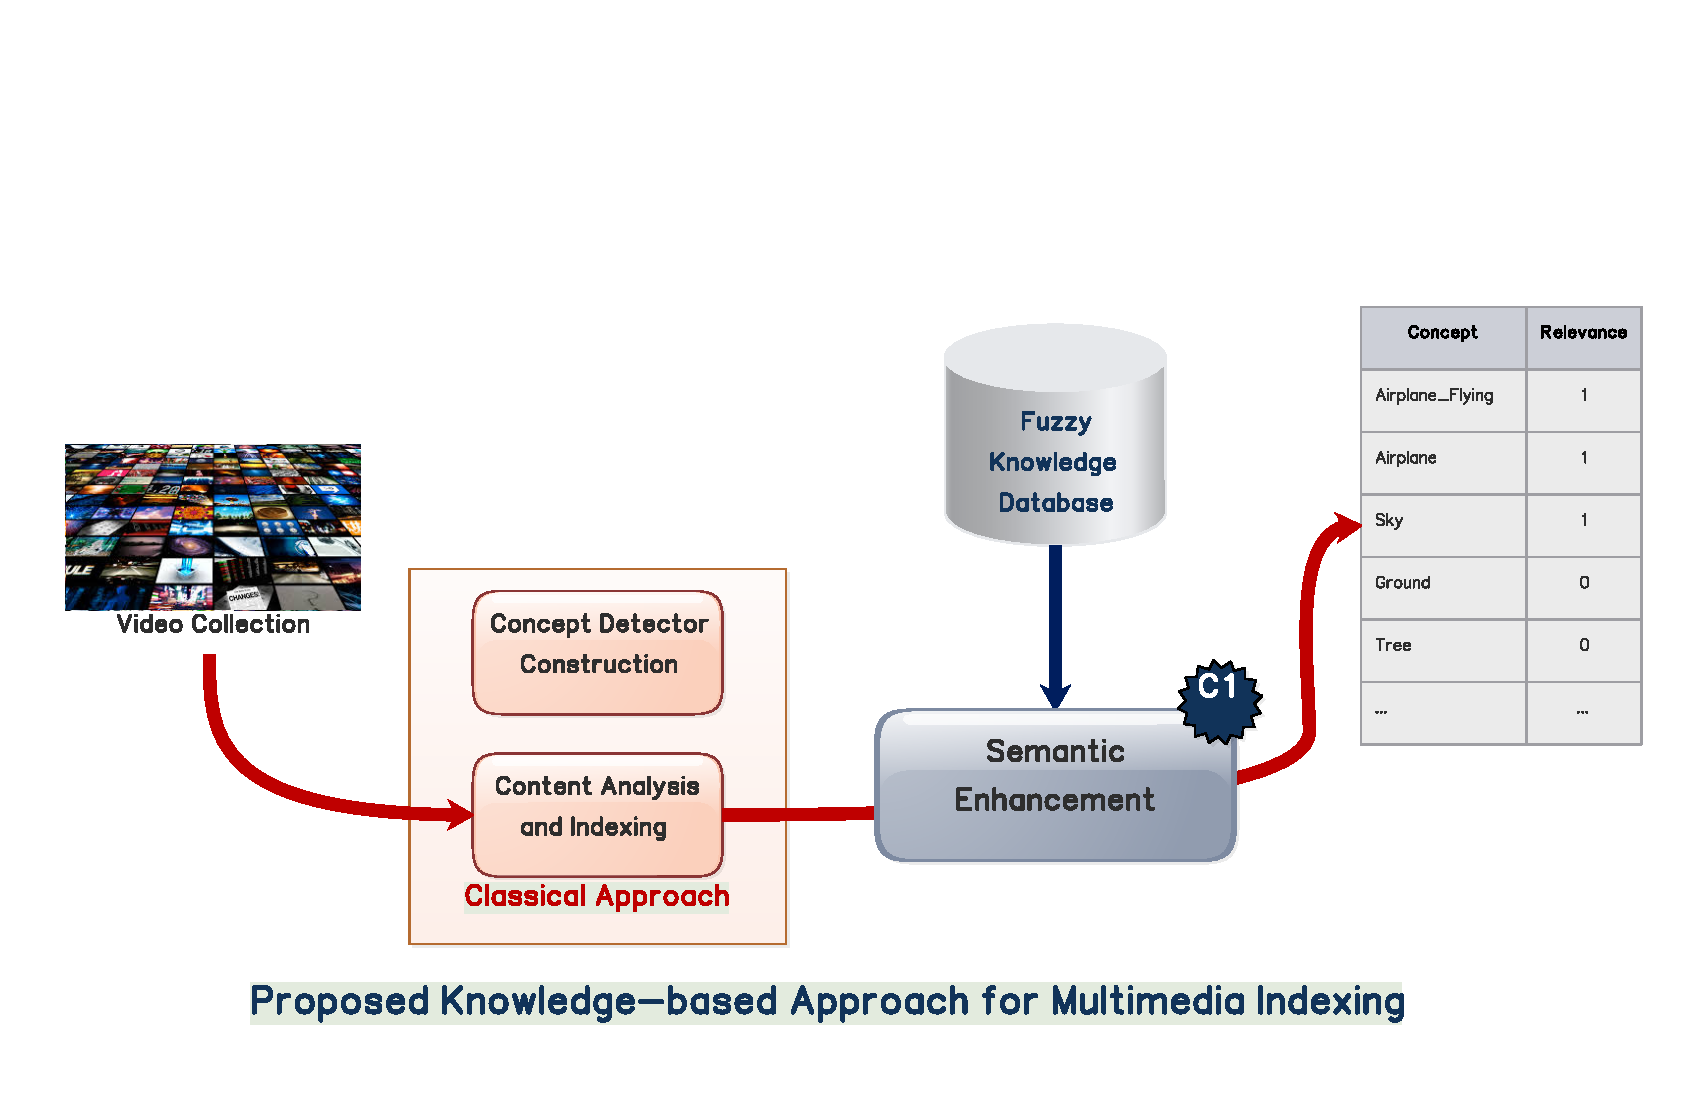
\includegraphics[scale=0.30]{graphics/contribution/contrib_overview_2} \end{center}

\end{frame}

\begin{frame}
	\frametitle{The JDL/Dfs data fusion model \citep{Waltz1990}}
	\only<1>{\hspace*{-1cm}\centering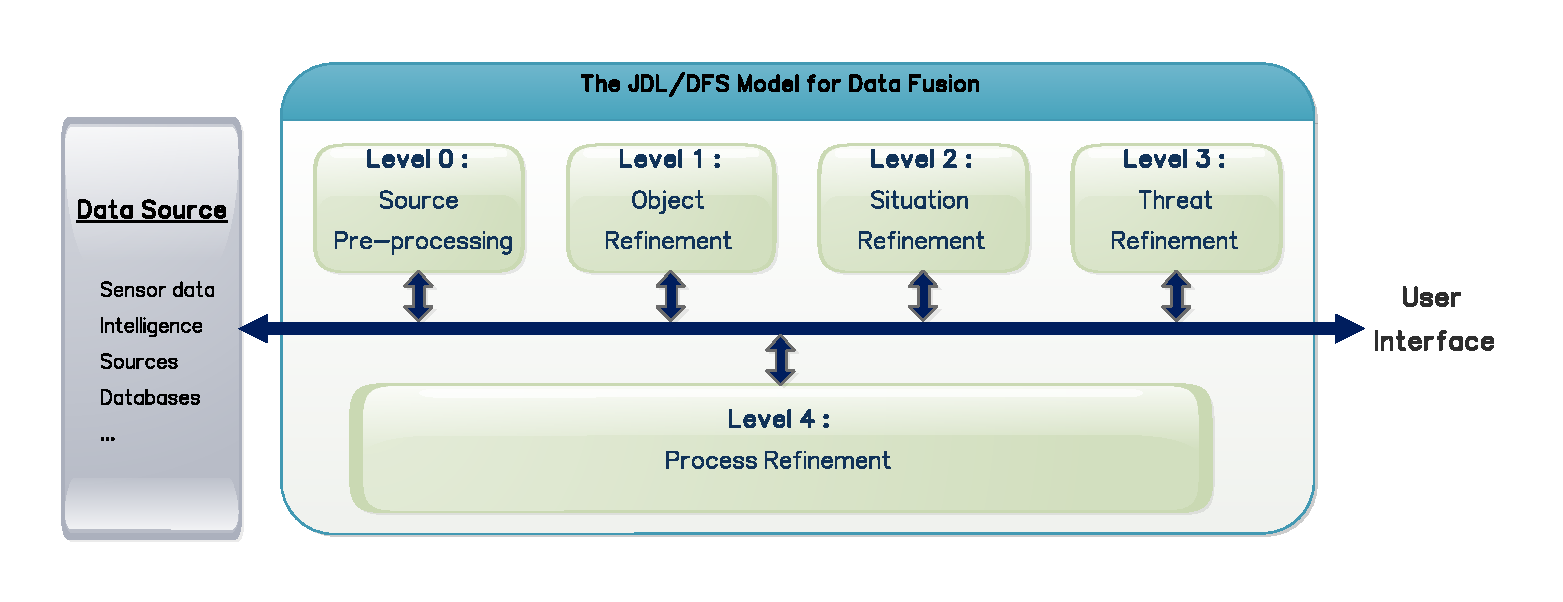
\includegraphics[scale=0.47]{graphics/c1/JDL}}
	\only<2>{\hspace*{-1cm}\centering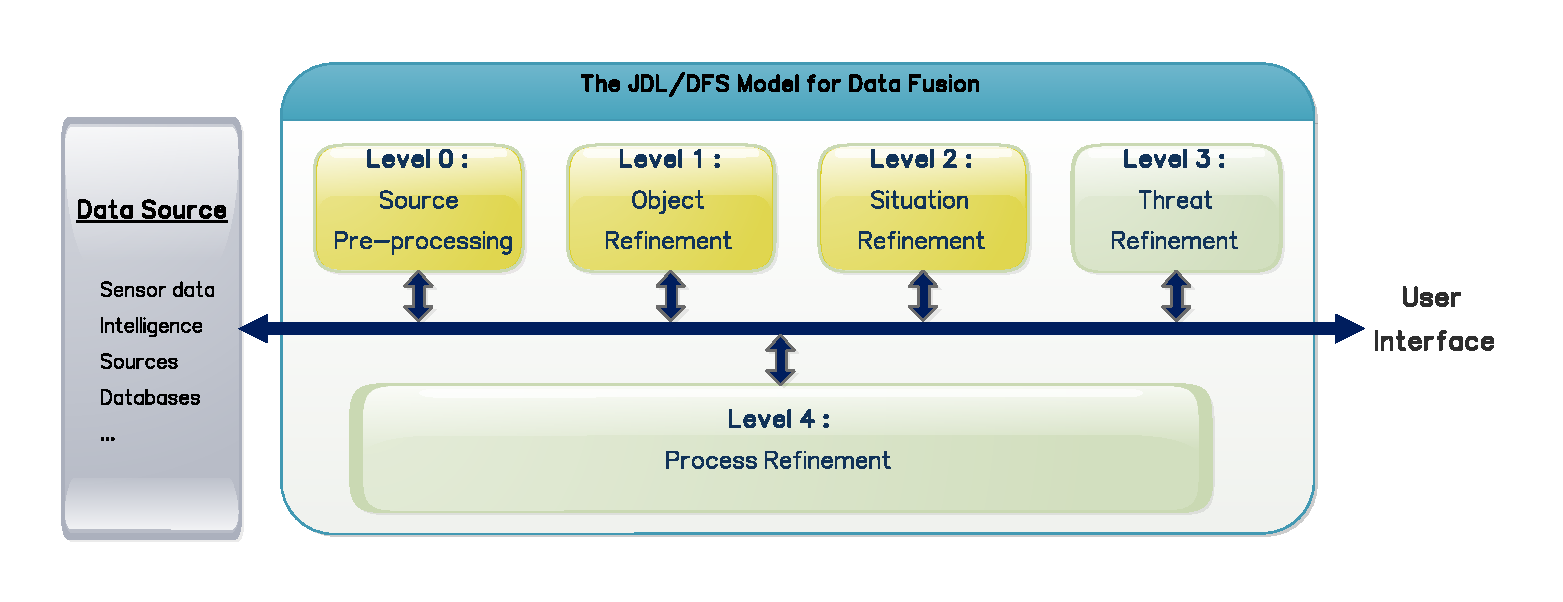
\includegraphics[scale=0.47]{graphics/c1/JDL2}}
\end{frame}
% \begin{frame}
% 	\frametitle{$C_{1}$: Proposed Approach}
	%\only<1>{\hspace*{-1cm}\centering
\includegraphics[scale=0.42]{graphics/c1/JDL_regimvid_1}}
	%\only<2>{\hspace*{-1cm}\centering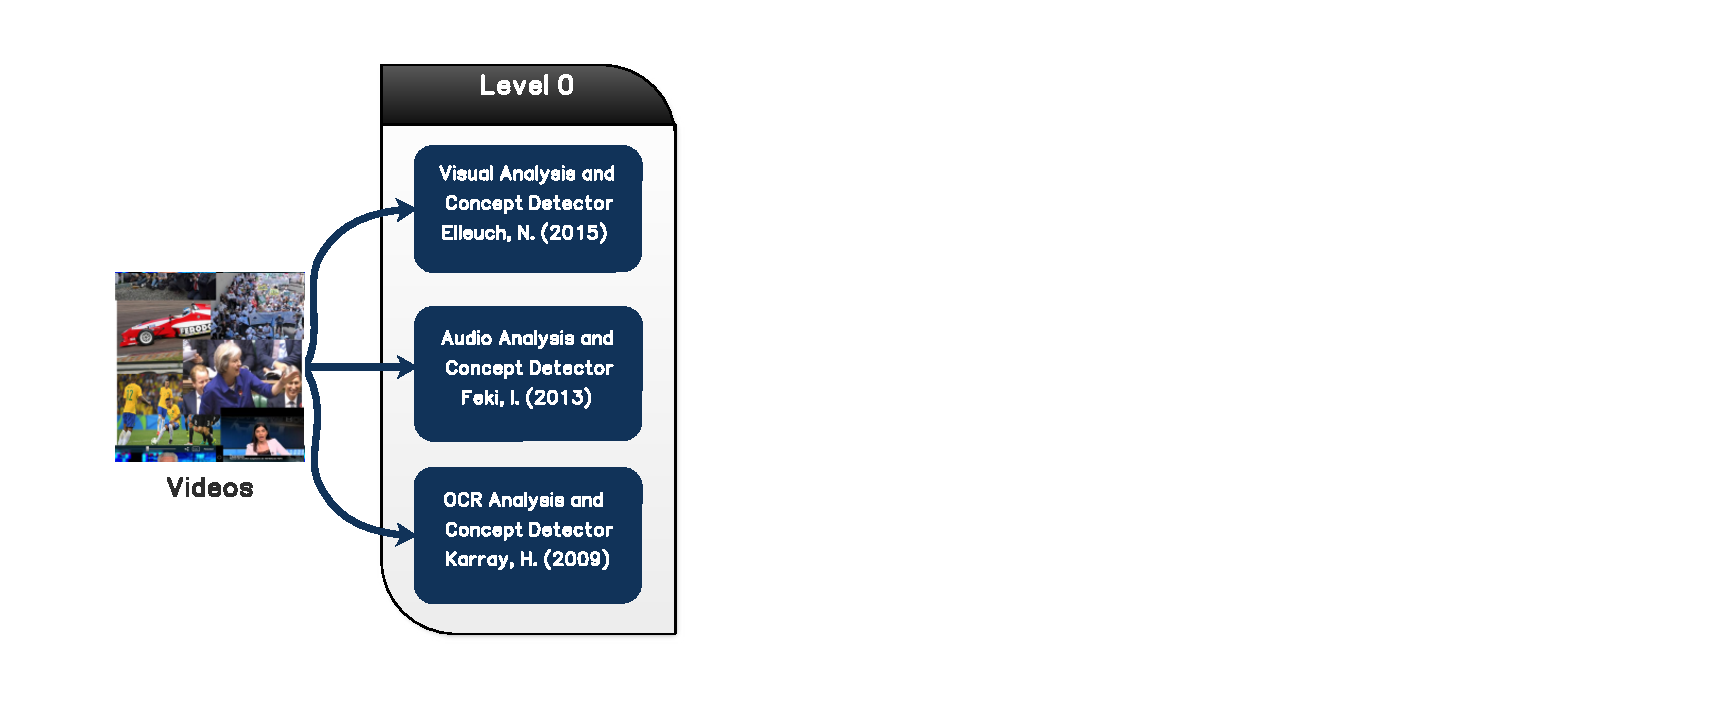
\includegraphics[scale=0.42]{graphics/c1/JDL_regimvid_2}}
	%\only<3>{\hspace*{-1cm}\centering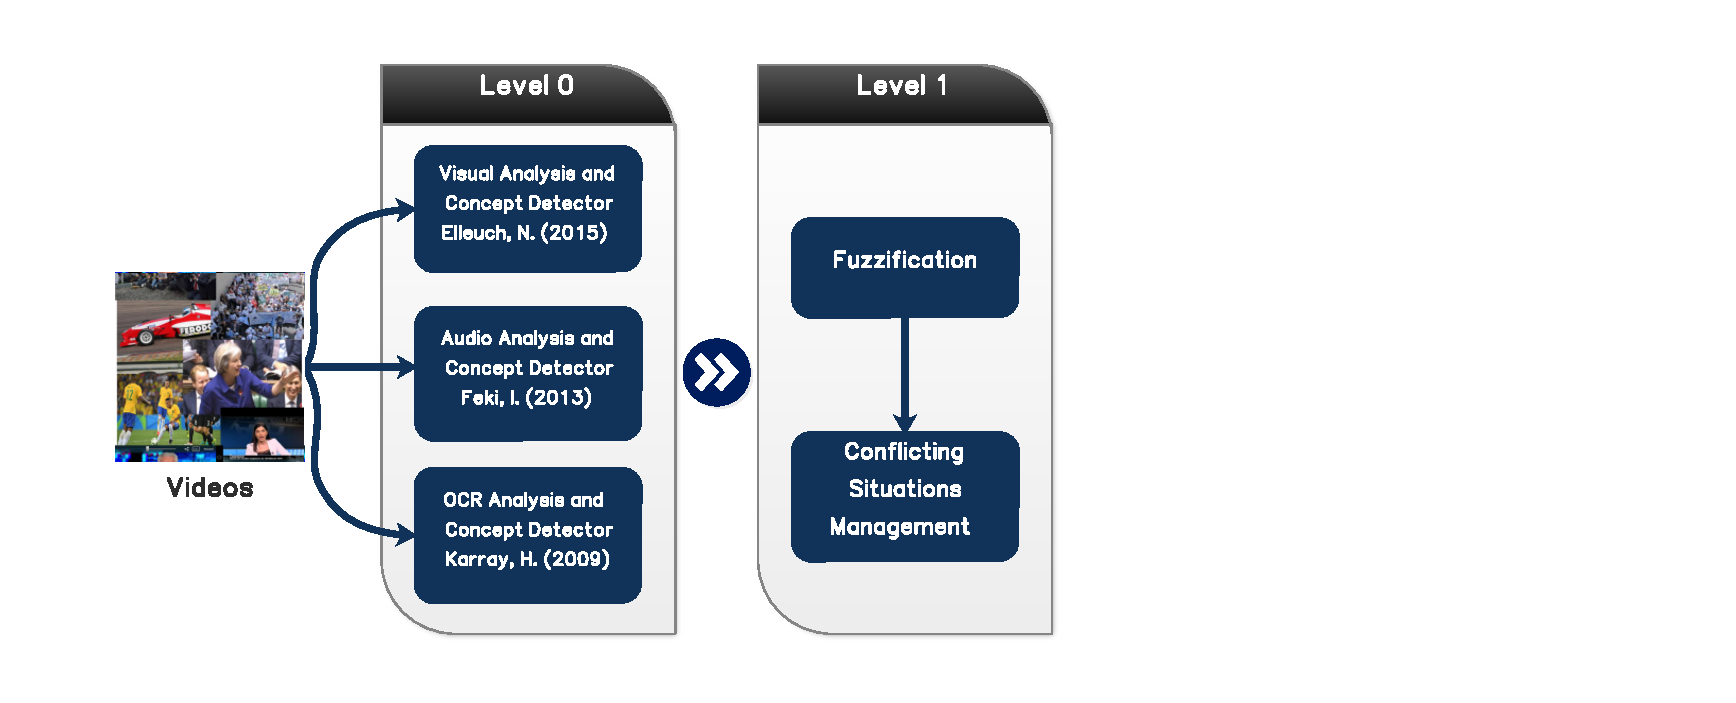
\includegraphics[scale=0.42]{graphics/c1/JDL_regimvid_3}}
% 	\only<4>{\hspace*{-1cm}\centering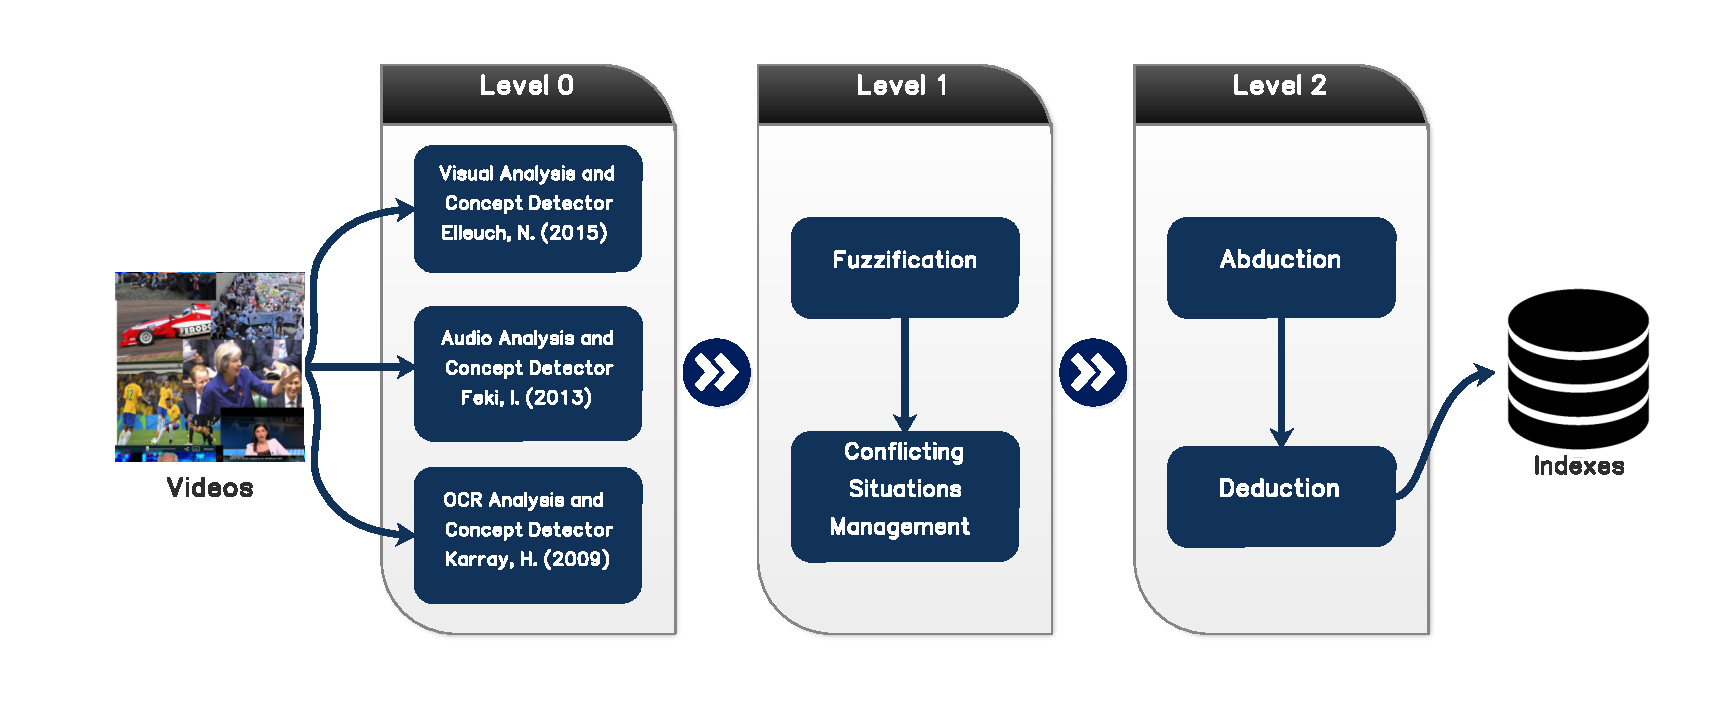
\includegraphics[scale=0.42]{graphics/c1/JDL_regimvid_4}}
%  	{\hspace*{-1cm}\centering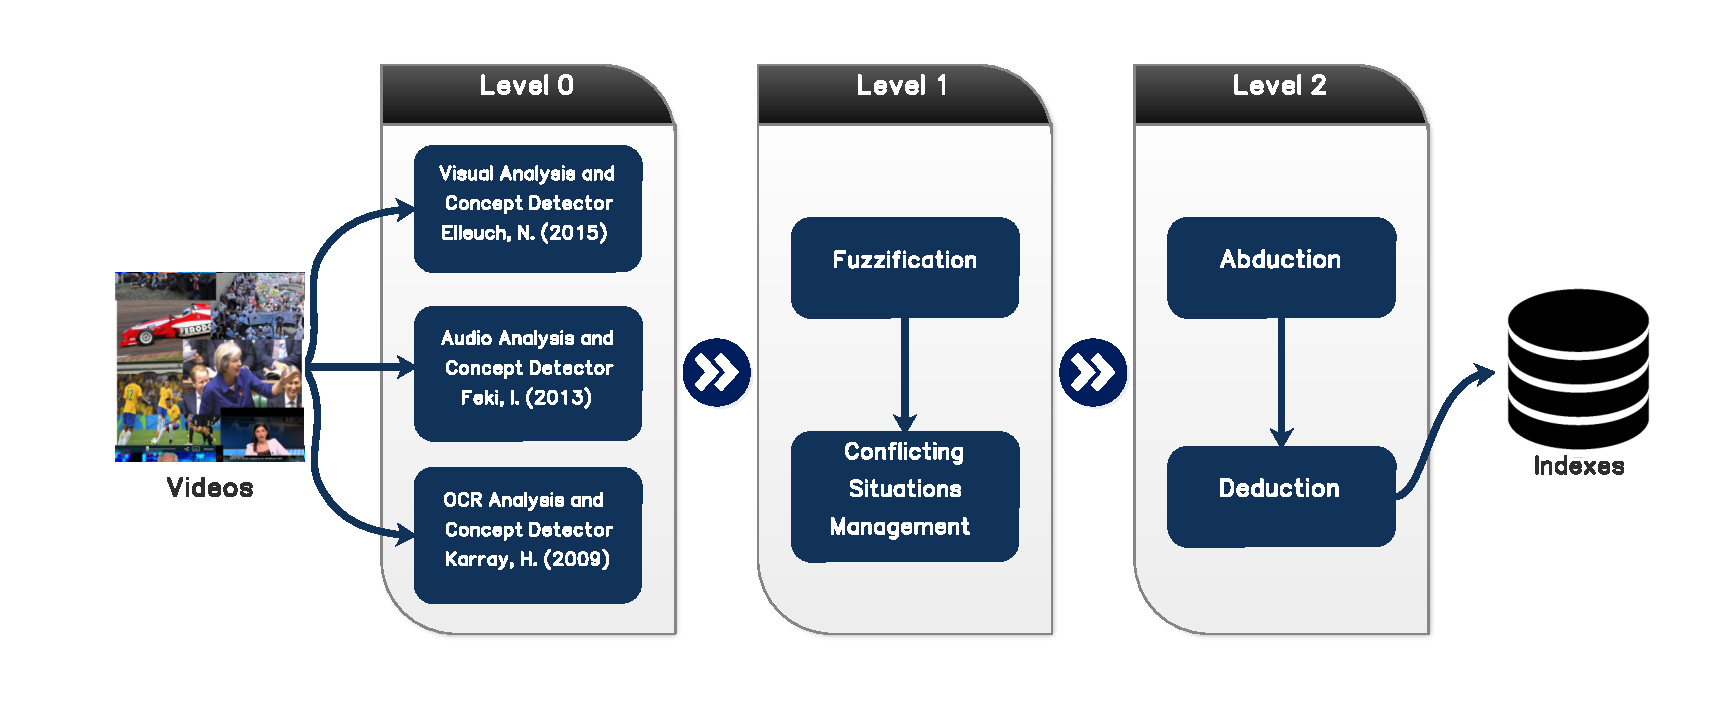
\includegraphics[scale=0.42]{graphics/c1/JDL_regimvid_4}}

% \end{frame}

\begin{frame}
	\frametitle{$C_{1}$: Proposed Approach - Level 0 (Pre-Processing)}
	\small
	\begin{block}{}
		\begin{itemize}
% 			\item Analyze the video content in order to identify semantic concepts
% 			\item The analyzed video is segmented into shots
% 			\item Each shot is labeled by a set of semantic concepts
			\item Level done within these thesis works:
				\begin{description}
					\item[Visual:] Elleuch, N. (2015)
					\item[Audio:] Feki, I. (2013)
					\item[Text/OCR:] Karray, H. (2009)
				\end{description}
		\end{itemize}
	\end{block}
	{\centering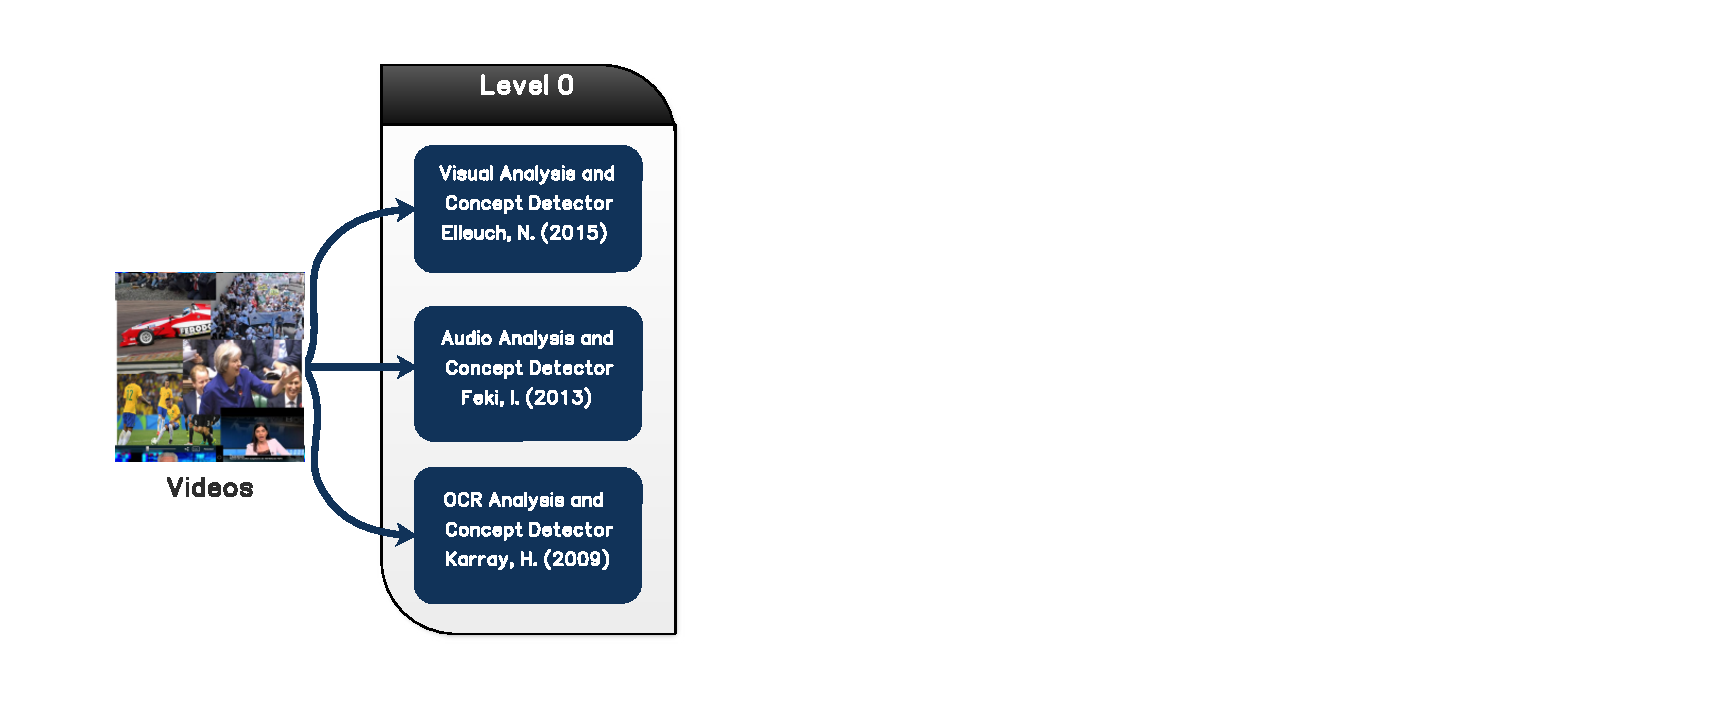
\includegraphics[scale=0.36]{graphics/c1/JDL_regimvid_2}}
\end{frame}

\begin{frame}
	\frametitle{$C_{1}$: Proposed Approach - Level 1 (Object Refinement)}
	\small
	\begin{block}{}
		\begin{description}
			\item[Step 1-Fuzzification:] Rank based fuzzification,
			\item[Step 2-Conflicting Situations Management:]
			       A confidence degree for each modality:
			       $\mu(c) = \alpha \mu_{1}(c) +  \beta \mu_{2}(c) +  \gamma \mu_{3}(c)$ \\where $\alpha + \beta + \gamma= 1$
		\end{description}
	\end{block}
	{\centering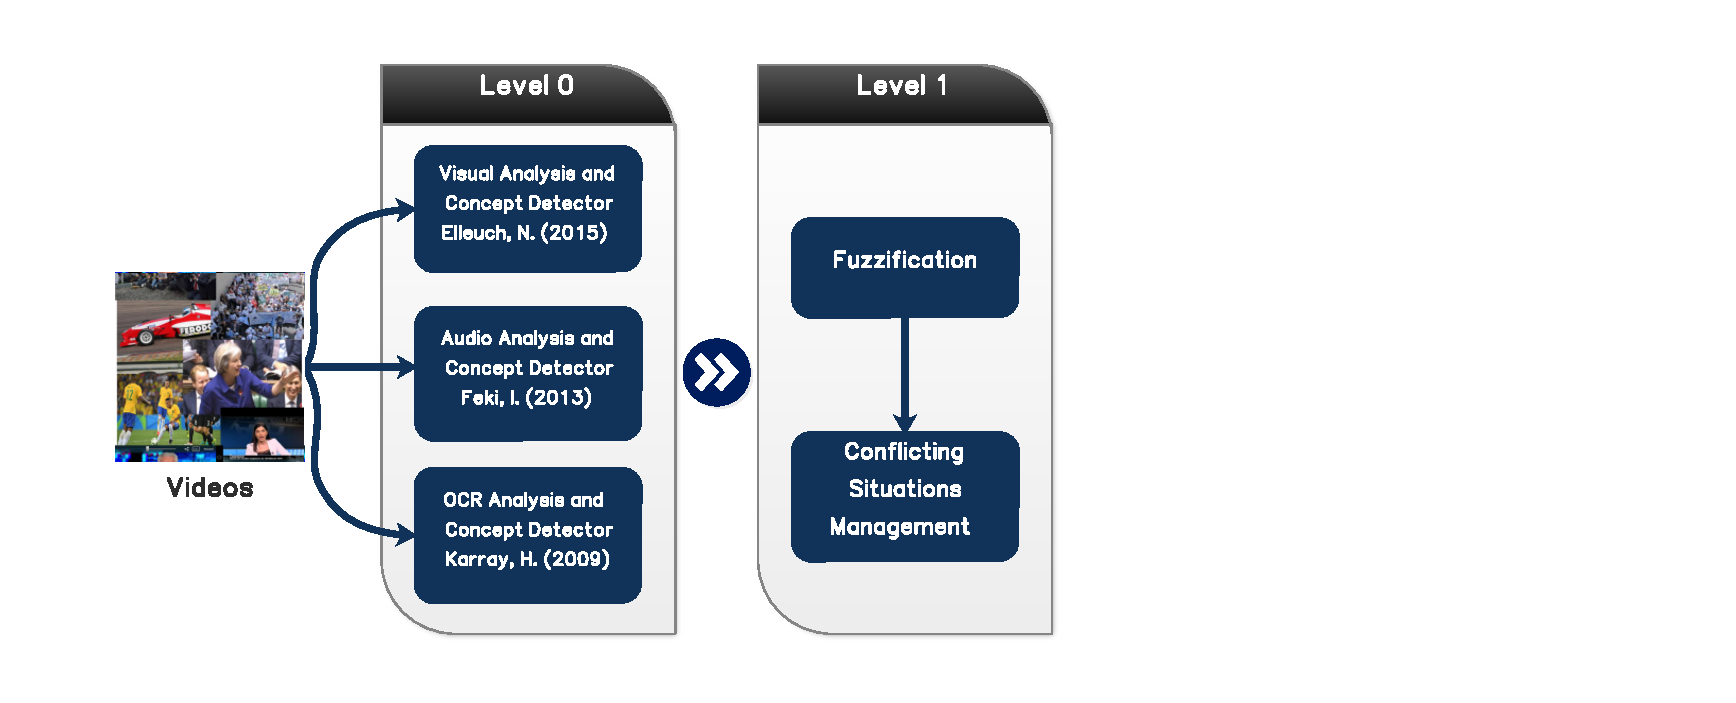
\includegraphics[scale=0.36]{graphics/c1/JDL_regimvid_3}}
\end{frame}

\begin{frame}
	\frametitle{$C_{1}$: Proposed Approach - Level 2 (Situation Refinement)}
	\small
	\begin{block}{}
		Avail of the knowledge dataset capabilities:
		\begin{description}
			\item[Abduction:] Looks for new valuable Knowledge,
			\item[Deduction:] Looks for implicit concepts by analyzing detected explicit ones.
		\end{description}
	\end{block}
	\only<1>{{\centering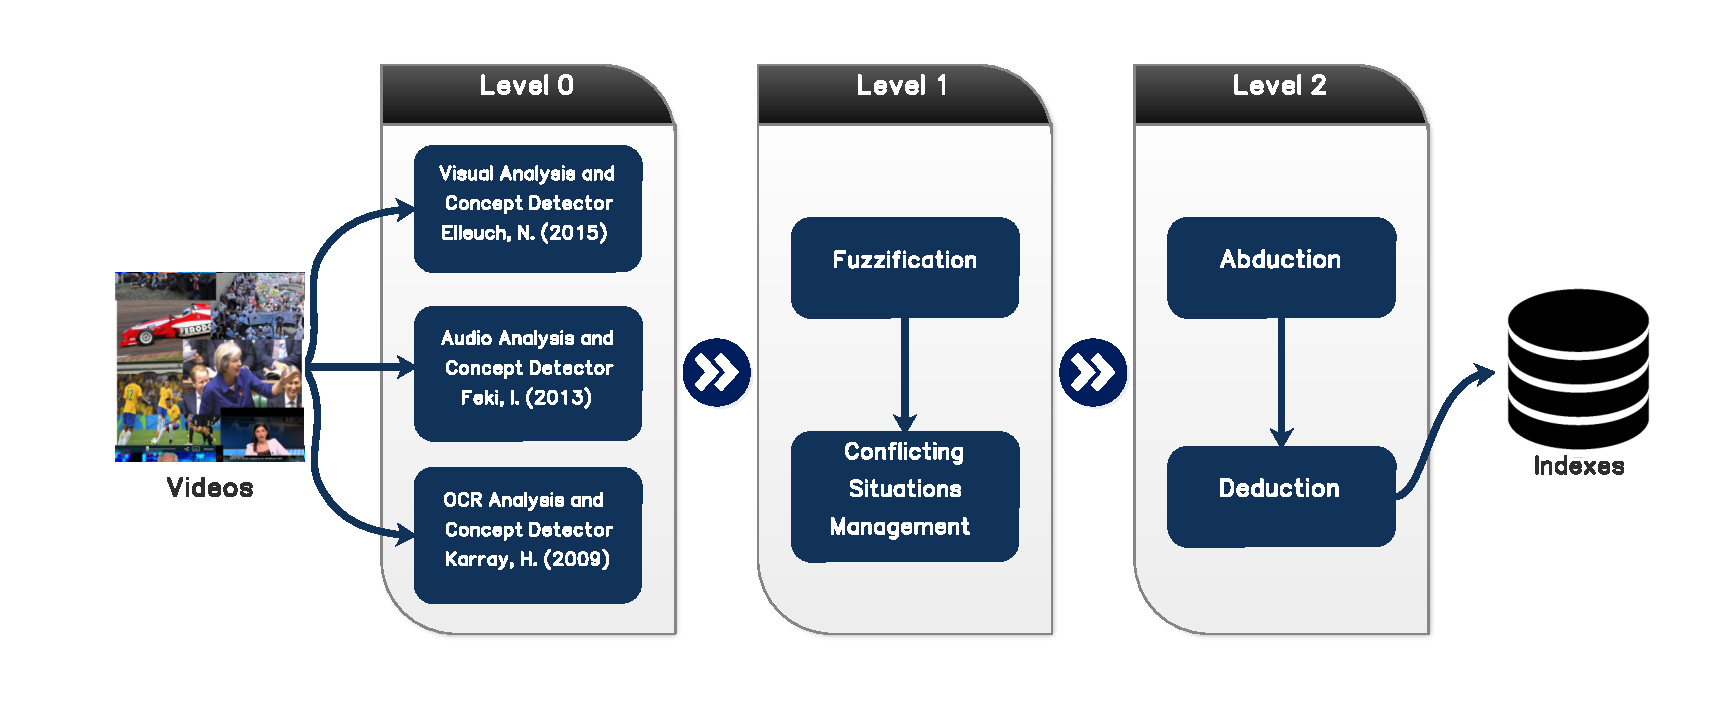
\includegraphics[scale=0.36]{graphics/c1/JDL_regimvid_4}}}
	\only<2>{\begin{columns}
  		\begin{column}{0.49\textwidth}
       		%\begin{block}{Deduction Engine}
			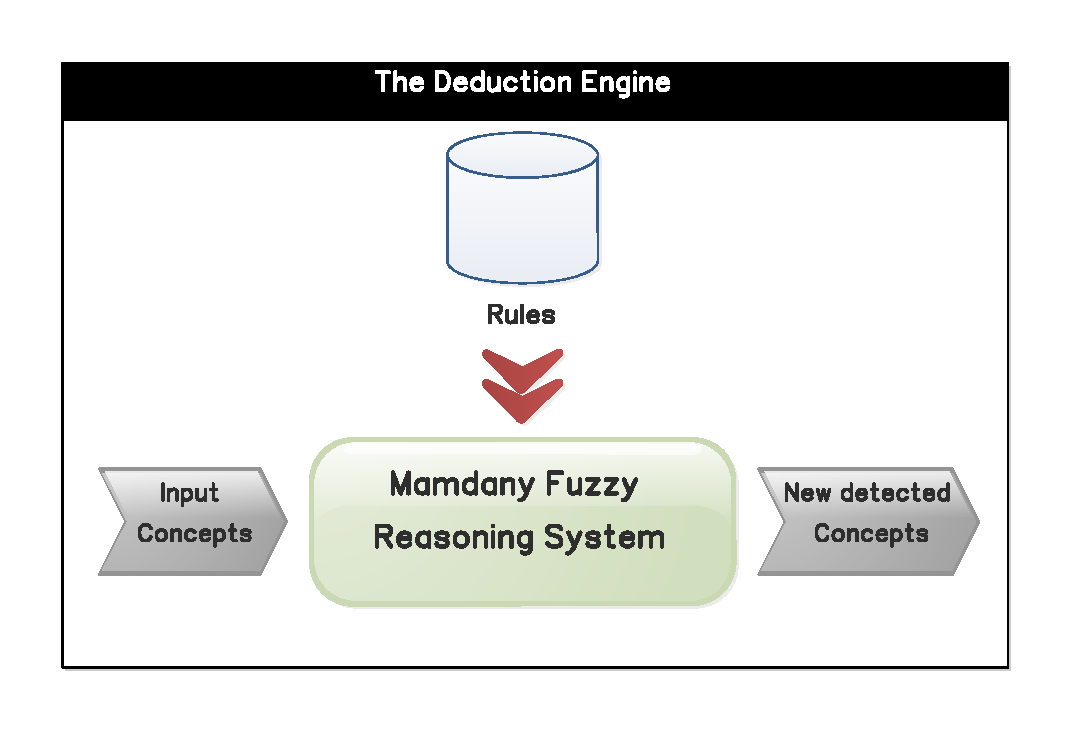
\includegraphics[scale=0.33]{graphics/c1/deduction}
		%\end{block}
    		\end{column}
    		\begin{column}{0.49\textwidth}
       		%\begin{block}{Abduction Engine}
			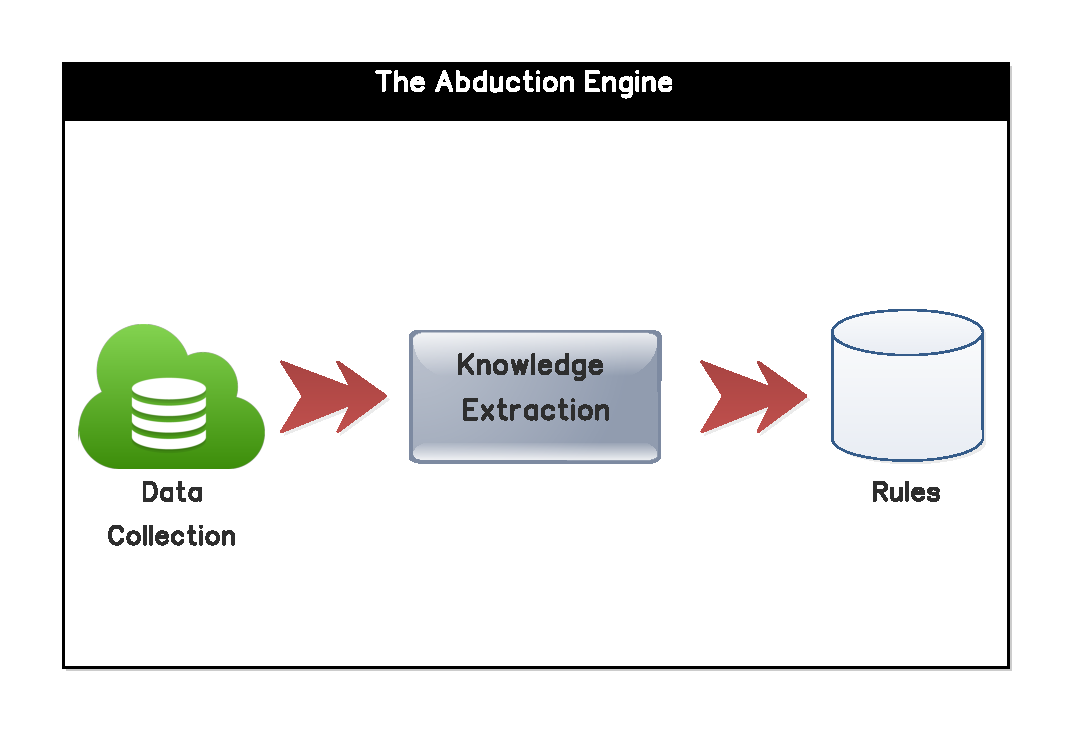
\includegraphics[scale=0.33]{graphics/c1/abduction}
		%\end{block}
    		\end{column}
	\end{columns}
	}
\end{frame}


\begin{frame}
	\frametitle{$C_{1}$: Preliminary Experiment I}
	\small
	\begin{exampleblock}{Experimentation Setup}
		\begin{itemize}
			\item \textsc{TrecVid 2010}: $200h$ of video development set and $200h$ of video test set
			\item 130 semantic concepts
		  \end{itemize}
	\end{exampleblock}

	\begin{exampleblock}{Baseline}
		\begin{itemize}
			\item We look to evaluate the semantic enhancement  of a non knowledge-based approach 
			\alert{\citep{Elleuch2010}}
			\item \alert{Visual} semantic indexing
			\item We used the \alert{\textsc{LsCom}} Ontology for the rules
		 \end{itemize}
	\end{exampleblock}
\end{frame}
\begin{frame}
	\frametitle{$C_{1}$: Preliminary Experiment II}
	\small
	{\only<1>{
	\begin{exampleblock}{Accuracy Evaluation}
		\centering
%			\includegraphics[scale=0.6]{graphics/c1_result1}
		\centering
		\tiny
		\begin{tabular}{|l||ccc|ccc|}\hline
				\multirow{1}{*}{\textit{\textbf{Semantic Concepts}}} & 	
				\multicolumn{3}{c}{\textbf{Baseline [Elleuch, N. (2015)]}} & 
				\multicolumn{3}{c|}{\textbf{\alert{Knowledge based}}}\\ 

				& infAP & P & R & infAP & P & R \\
				\hline
				\hline
	
				Outdoor	&	-&	0.52	&	0.59&	-&	\textbf{\alert{0.88}}	& \textbf{\alert{0.77}} \\
				Vegetation& 0.1 & 0.74		& 0.68& 0.1& 0.74 & 0.68  \\
				Landscape& -& 0.6		& 0.79& -& 0.6 & 0.79\\
				Sky& -& 0.66	& 0.9		& -& 0.66& 0.9  \\
				Trees& -& 0.62& 0.72 & - & 0.62 & 0.72\\
				Mountain& -& 0.68 & 0.8 & -  & 0.68 & 0.8  \\
				Ground\_Vehicle& 0.043  & 0.3& 0.66& \textbf{\alert{0.18}} & \textbf{\alert{0.6}} & \textbf{\alert{0.73}}\\
				Road& -& 0.43& 0.6 & -& 0.43& 0.6 \\
				Car  & 0.075 & 0.42 & 0.64& \textbf{\alert{0.17}} & \textbf{\alert{0.58}} & \textbf{\alert{0.73}} \\
				Bus& -& 0.52& 0.73& - & 0.52& 0.73 \\
				Bicycles& 0.142& 0.67& 0.92& \textbf{\alert{0.185}}& \textbf{\alert{0.82}}& \textbf{\alert{0.97}} \\
				Emergency Vehicle& -& 0.9& 0.83& - & 0.9& 0.83\\
				Building& 0.022& 0.18& 0.22& \textbf{\alert{0.1}}& \textbf{\alert{0.5}}& \textbf{\alert{0.43}}  \\
				Truck & -& 0.35& 0.37& -& 0.35& 0.37 \\
				Airplane Flying & 0.102& 0.8 & 0.78& 0.102& 0.8& 0.78                              \\
				Airplane  & -& 0.5& 0.6& -& \textbf{\alert{0.6}}& 0.6  \\
				\hline
		\end{tabular}
	\end{exampleblock}
	\footnotesize
		\begin{block}{}
			Semantic Enhancement of about \alert{$4.8\%$} compared to a classical concept detection [Elleuch, N. (2015)].
		\end{block}
	}}
	{\only<2>{
	\footnotesize
	\begin{exampleblock}{Teams}
		\alert{MediaMill} University of Amsterdam, \alert{PicSoM} University of Helsinki, \alert{Quaero} Europe, 
		\alert{FudaSys} Fuzhou University (China), \alert{Vireo} University of Hong Kong, \alert{IRIM} France, \alert{UC3M} University of Madrid, \dots{}
	\end{exampleblock}
	\begin{exampleblock}{}	
		\centering	
		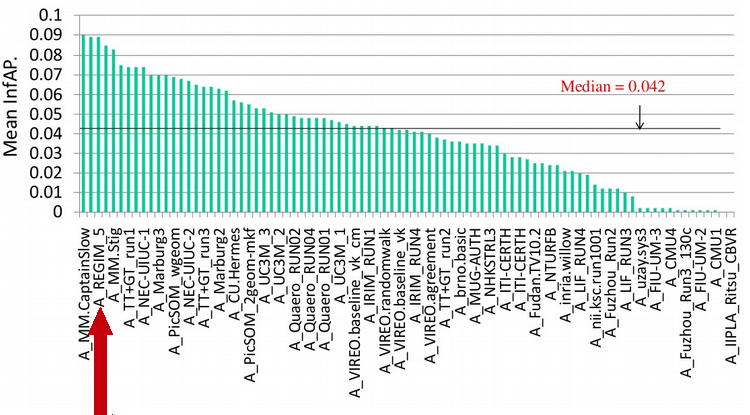
\includegraphics[scale=0.5]{graphics/c1/c1_result2}
	\end{exampleblock}
	}
	}

	
\end{frame}


\begin{frame}
	\frametitle{$C_{1}$: Fuzzy Contextual Ontology}
	\small
	\begin{block}{Motivation}
		\begin{itemize}
			\item Defining an \alert{ontology} more semantically richer than \textsc{LsCom},
			\item Introducing the semantic \alert{context}.
		  \end{itemize}
	\end{block}
	\begin{columns}
  		\begin{column}{0.45\textwidth}
       		\begin{block}{Deduction Engine}
			\begin{itemize}
				\item Defining a \alert{contextual space},
				\item \alert{relationships} between contexts and concepts,
				\item a \alert{deduction} engine is used to enhance a semantic interpretation.
			\end{itemize}
		\end{block}
    		\end{column}
    		\begin{column}{0.55\textwidth}
       		%\begin{block}{Abduction Engine}
			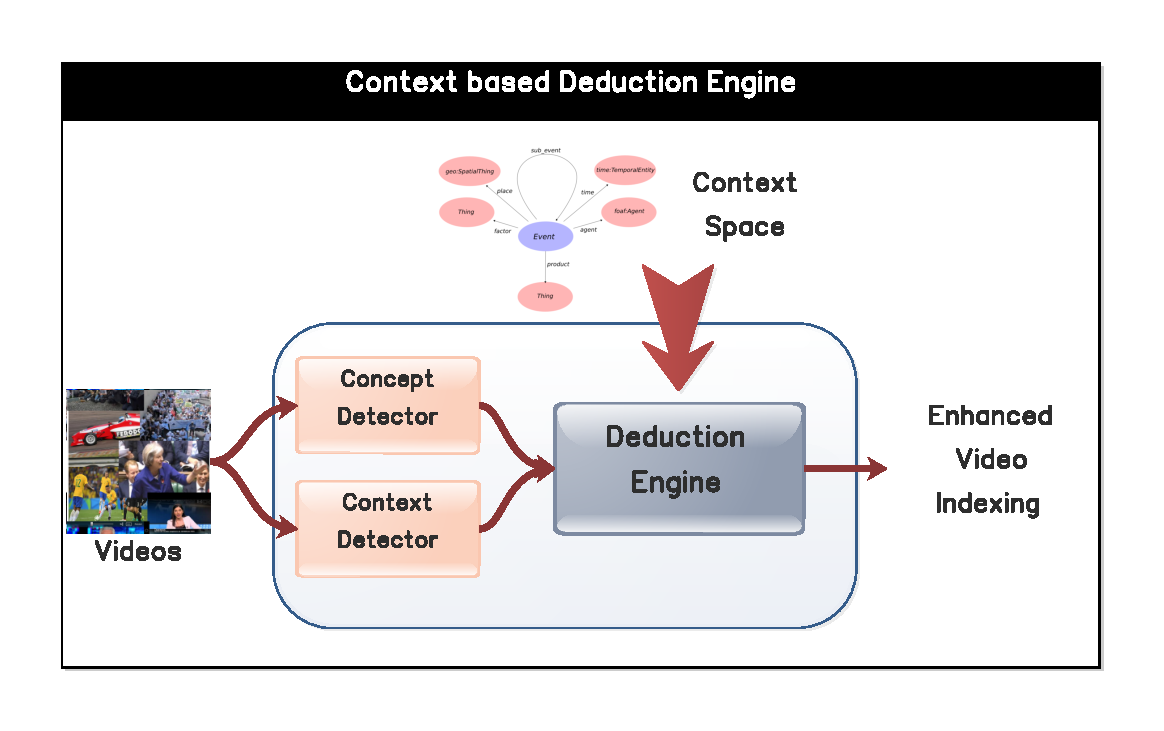
\includegraphics[scale=0.32]{graphics/c1/deduction_contexte}
		%\end{block}
    		\end{column}
	\end{columns}
\end{frame}

\begin{frame}
	\frametitle{$C_{1}$: Fuzzy Contextual Ontology (continued)}
	\footnotesize
	\begin{block}{$O^{f}$: a fuzzy Ontology}
		\begin{itemize}
			\item Let $T$ and $C$ be respectively a set of semantic contexts and concepts.
			\item Let $Q$ be a set of the fuzzy qualifiers: \alert{``weak''} and \alert{``strong''}. 
			\item We define four relationships :
			\begin{center} 
							\begin{tiny} 
							\begin{tabular}{c|c|c|c} 
								\hline\textbf{ \textit{Name}} & \textbf{\textit{Symbol}} & 
								\textbf{\textit{Meaning}} & \textbf{\textit{Type}} \\ 
					
								\hline Generalization & $t_{i}:t_{j} $ & 
								The concept $c_{i}$ is the generalization of the concept $c_{j} $ 
				 				&  $TxT$   \\ 
								
								\hline IsRelatedTo 	& $c_{i} |t{k}\rightarrow c_{j}$ &
								The concept $c_{i}$ is related to the concept $c_{j}$ within $t_{k}$ 
				 				& $CxC$  \\ 
					
								\hline IsPartOf 	& $\{c_{i}\} \in t_{j}	$ & 
								A set of concept $c_{i}$ is a part of the context $t_{j}$ 
								& $CxT$ \\ 
					
								\hline Includes 	& $t_{i} \supset c_{j}$	& 
								The context $t_{i}$ includes the concept $c_{j}$ 
				 				&  $TxC$ \\ 
								\hline 
							\end{tabular} 
							\end{tiny} 
							\end{center} 
		 \end{itemize}
	\end{block}
	%\pause
	\begin{block}{$O^{f}$: deduction engine}
		\begin{itemize}
			\item \alert{Strong Rule}: 
				$\alpha'_{k}(c_{j})=\mu_{k}*(max\{P(V_{S_{k}}|c_{i}),P(V_{S_{i}}|t_{k'})\})*\mu_{Strong}(\alpha_{k})$
			\item \alert{Weak Rule}: 
				$\alpha'_{k}(c_{j})=\mu_{k}*(min\{P(V_{S_{k}}|c_{i}),P(V_{S_{i}}|t_{k'})\})*\mu_{Weak}(\alpha_{k})$
		\end{itemize}
	\end{block}
\end{frame}

\begin{frame}
	\frametitle{$C_{1}$: Second Experimentation}
	\small
	\begin{exampleblock}{Experimentation Setup}
		\begin{itemize}
			\item \textsc{TrecVid 2010} dataset
		  \end{itemize}
	\end{exampleblock}
	\begin{exampleblock}{The $O^{f}$ ontology: Defined by Experts}
		\centering 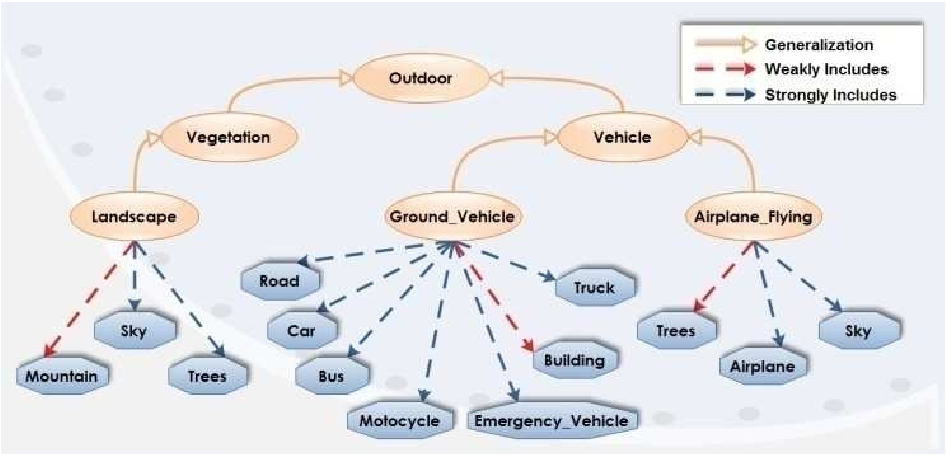
\includegraphics[scale=0.5]{graphics/c1/of}
	\end{exampleblock}
\end{frame}

\begin{frame}
	\frametitle{$C_{1}$: Obtained results with $O^{f}$}
	\centering
	\tiny
		\begin{tabular}{l||ccc|ccc|cc}\hline
				\multirow{2}{*}{\textit{\textbf{Semantic Concepts}}} & 	
				\multicolumn{3}{c}{\textbf{Concept Detector}} & 
				\multicolumn{3}{c}{\textbf{LSCOM}}&
				\multicolumn{2}{c}{\textbf{\alert{$O^{f}$}}}\\ 

				& infAP & P & R & infAP & P & R & P & R\\
				\hline
				\hline
	
				Outdoor	&-&0.52&0.59&-&	\textbf{0.88}& \textbf{0.77} & \textbf{\alert{0.9}} & \textbf{\alert{0.82}}\\
				Vegetation& 0.1 & 0.74& 0.68& 0.1& 0.74 & 0.68 & \textbf{\alert{0.93}} & \textbf{\alert{0.87}} \\
				Landscape& -& 0.6& 0.79& -& 0.6 & 0.79& \textbf{\alert{0.7}} & \textbf{\alert{0.82}}\\
				Sky& -& 0.66& 0.9& -& 0.66& 0.9 & \textbf{\alert{0.85}} & \textbf{\alert{0.95}} \\
				Trees& -& 0.62& 0.72 & - & 0.62 & 0.72 & \textbf{\alert{0.73}} & \textbf{\alert{0.82}}\\
				Mountain& -& 0.68 & 0.8 & -  & 0.68 & 0.8 & \textbf{\alert{0.83}} & \textbf{\alert{0.85}} \\
				Ground\_Vehicle& 0.043  & 0.3& 0.66& \textbf{0.18} & \textbf{0.6} & \textbf{0.73} 
								& \textbf{\alert{0.69}}&\textbf{\alert{0.75}}\\
				Road& -& 0.43& 0.6 & -& 0.43& 0.6 & \textbf{\alert{0.88}} & \textbf{\alert{0.9}} \\
				Car  & 0.075 & 0.42 & 0.64& \textbf{0.17} & \textbf{0.58} & \textbf{0.73} 
								& \textbf{\alert{0.79}} & \textbf{\alert{0.83}}\\
				Bus& -& 0.52& 0.73& - & 0.52& 0.73 &0.52 & 0.73\\
				Bicycles& 0.142& 0.67& 0.92& \textbf{0.185}& \textbf{0.82}& \textbf{0.97} & \textbf{\alert{0.83}} & 0.97\\
				Emergency Vehicle& -& 0.9& 0.83& - & 0.9& 0.83 & 0.9& 0.83\\
				Building& 0.022& 0.18& 0.22& \textbf{0.1}& \textbf{0.5}& \textbf{0.43} & \textbf{\alert{0.55}} & \textbf{\alert{0.45}} \\
				Truck & -& 0.35& 0.37& -& 0.35& 0.37 & 0.35 & 0.37\\
				Airplane Flying & 0.102& 0.8 & 0.78& 0.102& 0.8& 0.78 & \textbf{\alert{0.83}} & \textbf{\alert{0.79}}  \\
				Airplane  & -& 0.5& 0.6& -& \textbf{0.6}& 0.6  & \textbf{\alert{0.71}} & \textbf{\alert{0.69}}\\
				\hline
		\end{tabular}
		%\pause
		\footnotesize
		\begin{exampleblock}{}
			Semantic Enhancement of about \alert{$21\%$} compared to a classical concept detection.
		\end{exampleblock}
\end{frame}

\begin{frame}
	\frametitle{$C_{1}$: Related publications}
	\begin{block}{}
		{\tiny
		\begin{itemize}
			\item \citep{Elleuch2010} Elleuch, N., \textbf{Zarka, M.}, Feki, I., Ammar, A. B., 
				\&{} Alimi, A. M. (2010). REGIMVID at TRECVID2010: semantic 
				indexing. In P. Over et al. (Eds.), \emph{TRECVID 2010 workshop
				participants notebook papers, Gaithersburg, MD, USA, november 2010}. 
				National Institute of Standards and Technology (\alert{NIST}). 
				
			\item \citep{Zarka2011a} \textbf{Zarka, M.}, Ammar, A. B., \&{} Alimi, A. M. (2011). 
				Multimodal fuzzy fusion system for semantic video indexing. 
				In \emph{IEEE symposium on computational intelligence for multimedia,
				signal and vision processing, CIMSIVP 2011, Paris, France} (pp. 60--66). \alert{IEEE}.

			\item \citep{Elleuch2011} Elleuch, N., \textbf{Zarka, M.}, Ammar, A. B., \&{} Alimi, A. M. (2011). 
				A fuzzy ontology: Based framework for reasoning in visual video content analysis 
				and indexing. In Proceedings of the eleventh international 
				workshop on multimedia data mining (pp. 1--8). New York, NY, USA: \alert{ACM}.
				

			\item \citep{Ksentini2012} Ksentini, N., \textbf{Zarka, M.}, Ammar, A. B., \&{} Alimi, A. M. (2012). 
				Toward an assisted context based collaborative annotation. In P. Lambert (Ed.), 
				\emph{10th international workshop on content-based multimedia indexing, 
				CBMI 2012, annecy, france, june 27--29, 2012} (pp. 71--76). \alert{IEEE}.
				
		\end{itemize}
		}
	\end{block}	
\end{frame}
